
\chapter{Data}

\section{ Data Overview}
The dataset was generated in VK Lab with the aim of Identifying the gas by using a gas sensor of different types at different temperatures. A sensor array of 3 component metal oxides was used to identify the mixture's four distinct volatile organic compounds(VOCs). The metal oxide sensor array comprises NiO-Au(ohmic), CuO-Au(Schottky), and ZnO-Au(Schottky) sensors made by DC reactive sputtering method and having a thickness of 80-100nm. This array was subject to various VOC concentrations, including ethanol, acetone, toluene, and chloroform, one by one and in a pair of gases \cite{singh2024metal}. The dataset consists of about 22 lac data points with features/variables such as Resistance, Sensor, Gas Concentration, Temperature, and Gas. The last one is the target variable. By using some suitable ML classification for Multiclass Classification, the models were trained to identify the Gas(Target Variable).
\begin{figure}
    \centering
    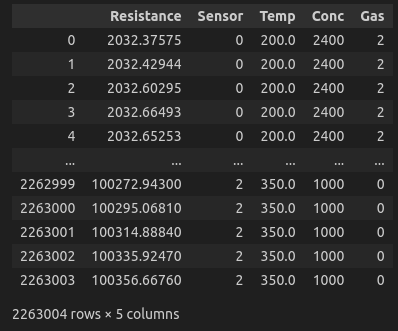
\includegraphics[width=0.5\linewidth]{Thesis Prashant//Images//Results/Screenshot from 2024-04-05 13-49-43.png}
    \caption{Data Head}
    \label{fig:enter-label}
\end{figure}

The resistance column has a range of order 2 to 6; the sensor column consists of three different types of sensors: NiO, CuO, and ZnO. The Temperature column consists of three unique values. 
[2400, 2100, 1800, 1500, 1200,  600,  300,  500,  100,   50,   20,
         10,    5,    2, 2500, 2000, 1000, 2700, 1900, 1700, 1550, 1370,
       1600, 1400,  900,  720,  540,  360,  180,   90,   30] These were the concentration used for sensing in the Conc column.
      The Last column is the target column, which has four types of gases: ethanol, acetone, toluene, and chloroform.

\begin{table}
    \centering
    \caption{Data Overview}
    \begin{tabular}{|c|c|c|c|c|c|}
    \hline
         & \textbf{Resistance} & \textbf{Sensor}  & \textbf{Temp } & \textbf{Conc} & \textbf{Gas}\\
         \hline
        % count & 2.263004e+06 & 2.263004e+06 & 2.263004e+06 & 2.263004e+06 & 2.263004e+06\\
       %  mean  & 2.030207e+05 & 1.146327e+00 & 6.368142e-01 & 1.951900e+01 & 1.429124e+00\\
         %std	&3.152512e+05 & 7.952693e-01 & 9.042883e-01 & 4.789999e+00 & 1.270319e+00\\
         \textbf{min}&8.655768e+02 & 0.000000e+00 & 0.000000e+00 & 0.000000e+00 & 0.000000e+00\\
       %  25\%	&5.910213e+03 & 0.000000e+00 & 0.000000e+00 & 1.600000e+01 & 0.000000e+00\\
        % 50\%	&1.113043e+05 & 1.000000e+00 & 0.000000e+00 & 1.900000e+01 & 1.000000e+00\\
       %  75\%	&2.332103e+05 & 2.000000e+00 & 2.000000e+00 & 2.400000e+01 & 3.000000e+00\\
         \textbf{max}&1.480000e+06 & 2.000000e+00 & 2.000000e+00 & 3.000000e+01 & 3.000000e+00\\
         \hline
    \end{tabular}
    \label{tab:my_label}
\end{table}


\section{Prepossessing Data}
So, our dataset has a total of five columns, the last of which is the target column. Since it is not a numerical attribute and we also want to classify them, it is necessary to hot encode the labels in the target column. so, inside the Gas column (target column) we have
'Gas' encoding: 
         Unique values:  ['Acetone' 'Chloroform' 'Ethanol' 'Toluene']
         Encoded labels:  [0 1 2 3]

and the sensor also has a non-numerical attribute therefore hot encoding is needed\\
'Sensor' encoding: 
         Unique values:  ['CuO' 'NiO' 'ZnO']
         Encoded labels:  [0 1 2] 

Data Processing with one hot encoding for target labels, resistance, and other features was scaled using a min-max scalar in zero to one range. Missing values in the dataset may result in bad model training, so using the mean method to find missing values was also added. Now, the data set has all the numerical values.

To train any model on a dataset, we need to shuffle and split it. Here, $80\%$ of data was used to train the model and $20\%$ of data was kept as a completely new unknown dataset to verify the model externally. That $80\%$ of the data was further used for supervised learning with a train-test split to the same ratio.
Just to see if there are extreme fluctuations in the resistance column, the percentile plot(Fig 2.2) was made. A K-density plot was used to visualize how each gas was distributed.Fig(2.3)

\begin{figure}
    \centering
    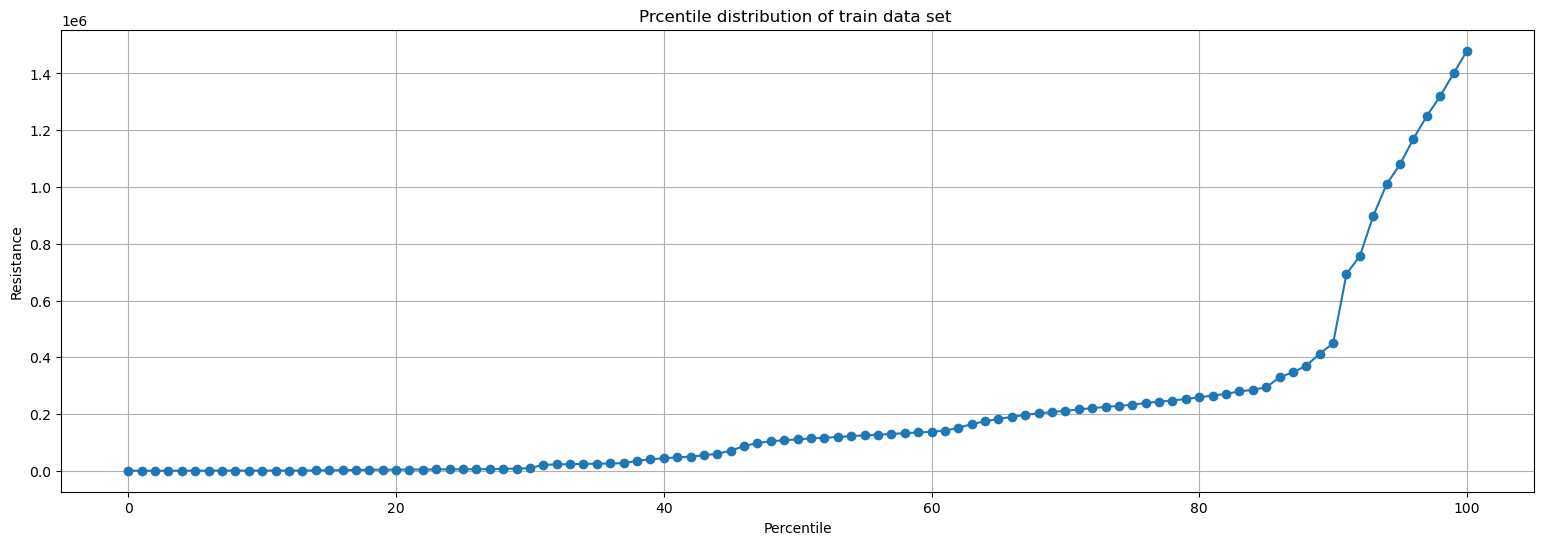
\includegraphics[width=1\linewidth]{Thesis Prashant//Images//Results/percentile plot of data.png}
    \caption{Percentile Plot}
    \label{fig:enter-label}
\end{figure}
\begin{figure}
    \centering
    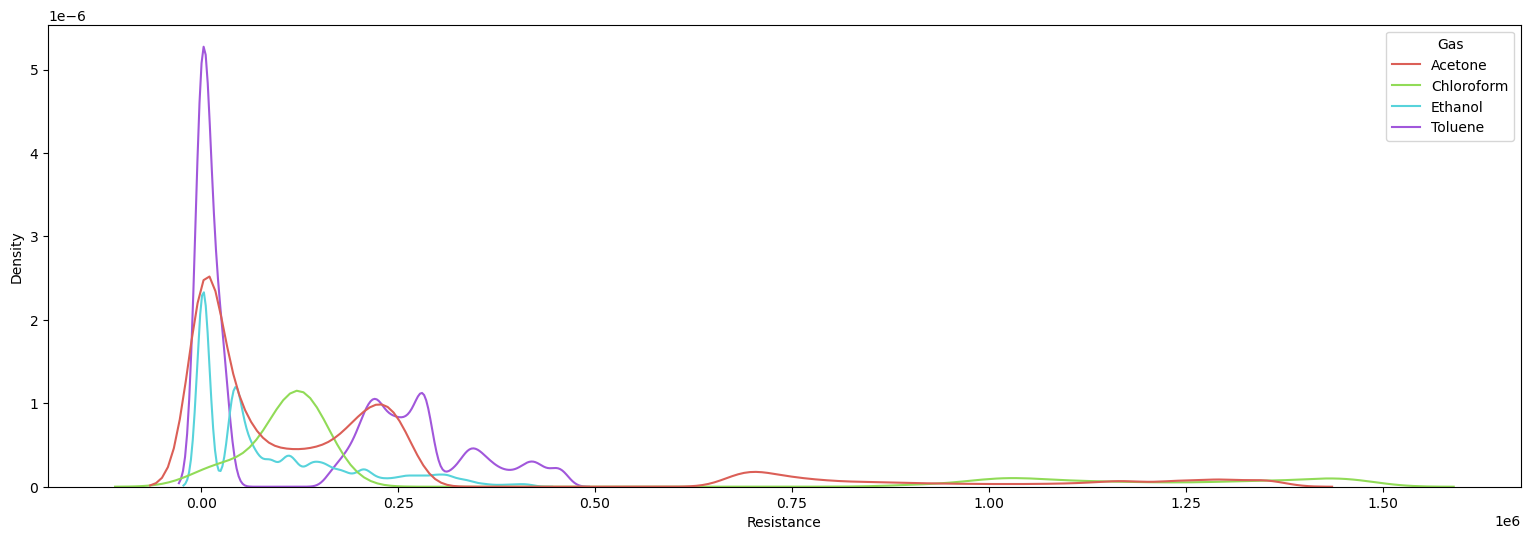
\includegraphics[width=1\linewidth]{Thesis Prashant//Images//Results/KD Plot .png}
    \caption{K-Density Plot of dataset}
    \label{fig:enter-label}
\end{figure}